\section{AutoEncoders}\label{sec:autoencoder}
Autoencoders are a form of explicit density estimators. In essence an
autoencoder tries to learn a latent space that can regenerate the images that it
takes as input. Once the network has been sufficiently trained the network can
recreate samples from the original dataset. Figure~\ref{fig:ae} shows the
general form of an autoencoder.

\begin{figure}[ht]
\centering
\includegraphics[width=0.48\textwidth]{autoencoder.png}
\caption{Autoencoder architecture}
\label{fig:ae}
\end{figure}

More formally an autoencoder seeks to map a sample $x$ to a latent variable $z$
where $x\in\mathbb{R}^n$ and $z\in\mathbb{R}^m$ and $n<m$. An autoencoder is a
one of the most simple architectures because we can simply take the mean square
error (MSE) between the generated image and the one trained on, making the
autoencoder an unsupervised learner. The encoding section of the network is only
needed for training. The drawback of the autoencoders is that they can not
generate new and unique samples. 

\section{Variational AutoEncoders}\label{sec:vae}
The Variational Autoencoder (VAE) is a small twist on autoencoder that allows
for a variation on data, allowing for the generation of unique samples. The
problem is that we want to learn the conditional probability 
$p(z|x) =\frac{p(x|z)p(z)}{p(x)}$ but $p(x) = \int p(x|z)p(z)dz$ is often
intractable. Instead a VAE learns an approximate function $q(z|x)$ that is
tractable. Because this function is different we need to introduce the
Kullback-Leibler (KL) divergence~\ref{eq:kl} to the regularization function, in
addition to the MSE. Additionally VAEs use a reparamerization trick because we
cannot backprop through stochastic nodes. To do this $\mu$ adn $\sigma$ are held
constant and $z$ becomes $z=\mu + \sigma\odot\epsilon$ and $\epsilon$ is allowed
to vary.

\begin{equation}
D_{KL}(P||Q) = \int P(x)\log\left(\frac{P(x)}{Q(x)}\right)dx
\label{eg:kl}
\end{equation}

By making these additions to the autoencoder the VAE is able to generate
variational data and actually learn the density of the dataset. An example of
the VAE architecture is shown in Figure~\ref{fig:vae}.

\begin{figure}[ht]
\centering
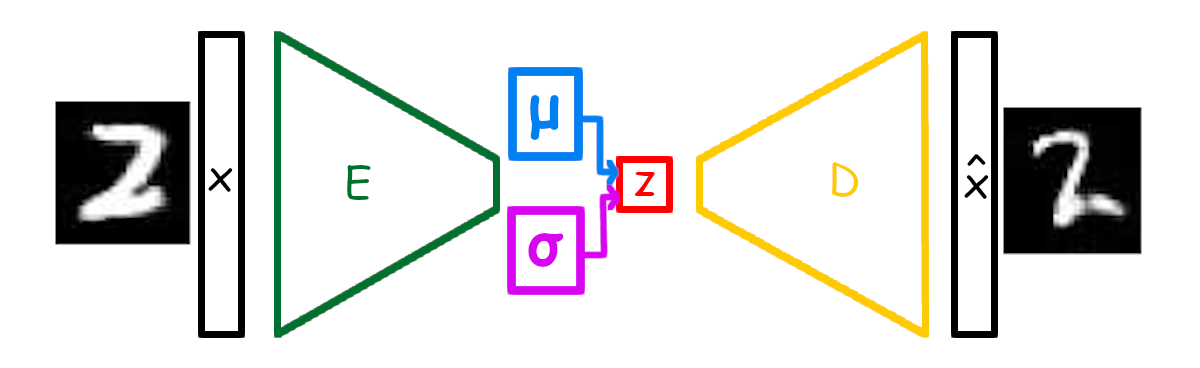
\includegraphics[width=0.48\textwidth]{VAE.png}
\caption{Autoencoder architecture}
\label{fig:vae}
\end{figure}
